\documentclass{beamer}
%\usetheme{default}    
\usepackage{graphicx}

\usetheme{Berkeley}    
\usecolortheme{crane}

\title{Consistency in the Cloud II}
\subtitle{Consistency v. Latency in Geo-Replicated Systems}
\author{Satabdi Aditya and Shannon Harwick}
\institute{University of Illinois at Chicago}
\titlegraphic{}
\date{\today}

\begin{document}


% --------------------------------------------------- Slide --0

\section{Li et al.} 

\begin{frame}
\frametitle{Paper 1: Li et al.}

\textbf{Title} Making Geo-Replicated Systems Fast as Possible,Consistent when necessary\newline
\textit{10th USENIX Symposium on Operating Systems Design and Implementation} \newline
Authors\newline
Date\newline

\end{frame}

% --------------------------------------------------- Slide --1

\begin{frame}
\frametitle{Motivation:}
\begin{enumerate}
\item To improve user-experience, services replicate  system state across geographical diverse sites.
\item Performance vs Consistency
\begin{itemize}
\item Amazon\'s Dynamo - eventual consistency where state temporarily diverge.
\item Yahoo PNUTS - avoids state divergence by requiring all operations that update the service state to be funneled through a primary site and thus incurring increased latency.
\end{itemize}
\end{enumerate}

\end{frame}


% --------------------------------------------------- Slide --2

\begin{frame}
\frametitle{Overview:}
\begin{enumerate}
\item RedBlue Consistency - Blue operations execute locally and are lazily replicated.Red operations are serialized with respect to each other and are immediately cross-site coordinated.
\item Conditions under which operations must be colored red or blue.
\item Decomposing operations into two components - a generator operation and a shadow operation.
\end{enumerate}

\end{frame}


% --------------------------------------------------- Slide --3

\begin{frame}
\frametitle{Properties of Geo-Replicated Systems}
\begin{enumerate}
\item Low latency - Operations should proceed after contacting a small number of users.
\item Causality - Monotonicity of user request within session and also preserving causality across clients
\item State Convergence - All replicas have executed the same set of operations
\item All operations should return a single value.
\item The system should provide a set of stable histories and support for general operations.
\item The system should preserve a set of invariants.
\item Eventual Propagation
\end{enumerate}
\end{frame}
% --------------------------------------------------- Slide --4

\begin{frame}
\frametitle{Related Work: Target end-to-end Properties}
\begin{figure}[t]
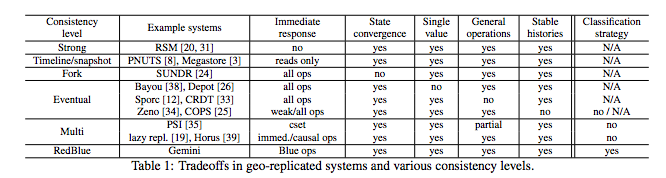
\includegraphics[width=10cm]{pic1.jpg}
\centering
\end{figure}
\end{frame}

% --------------------------------------------------- Slide --5

\begin{frame}
\frametitle{Related Work: Strong vs Weak Consistency}
\begin{enumerate}
\item
\end{enumerate}

\end{frame}


% --------------------------------------------------- Slide --6

\begin{frame}
\frametitle{Related Work: Other}
\begin{enumerate}
\item
\end{enumerate}

\end{frame}


% --------------------------------------------------- Slide --7

\begin{frame}
\frametitle{System Model}
\begin{enumerate}
\item
\end{enumerate}

\end{frame}

% --------------------------------------------------- Slide --8

\begin{frame}
\frametitle{RedBlue Consistency}
\begin{enumerate}
\item
\end{enumerate}

\end{frame}


% --------------------------------------------------- Slide --8

\begin{frame}
\frametitle{RedBlue Consistency - Definition}
\begin{enumerate}
\item
\end{enumerate}

\end{frame}

% --------------------------------------------------- Slide --8

\begin{frame}
\frametitle{State Convergence and RedBlue Bank}
\begin{enumerate}
\item
\end{enumerate}

\end{frame}

% --------------------------------------------------- Slide --9

\begin{frame}
\frametitle{Replicating side effects - Defining shadow operations}
\begin{enumerate}
\item
\end{enumerate}

\end{frame}

% --------------------------------------------------- Slide --10

\begin{frame}
\frametitle{Revisiting RedBlue consistency}
\begin{enumerate}
\item
\end{enumerate}

\end{frame}



%%% BEGIN SHANNON SECTION %%%
% --------------------------------------------------- Slide --

\section{Lloyd et al.} 

\begin{frame}
\frametitle{Paper 2: Lloyd et al.}

\textbf{Stronger Semantics for Low-Latency Geo-Replicated Storage} \newline
\textit{Proceedings of the 10th USENIX Symposium on Networked Systems Design and Implementation (NSDI’13)} \newline
Wyatt Lloyd, Michael J. Freedman, Michael Kaminsky, and David G. Andersen \newline
April 2013 \newline

\end{frame}

% --------------------------------------------------- Slide --
\begin{frame}
\frametitle{Motivation}
\begin{itemize}

\item Consider an example from Facebook
\pause\item Joe performs 2 actions:
	\begin{itemize}
		\pause\item Defriend boss.
		\pause\item Make snarky comment about boss and promise to quit.
	\end{itemize}
\pause\item In an \textcolor{red}{eventually} consistent system, these can be viewed in the wrong order for a period time, earning Joe his first unemployment check.
\pause\item This won't happen with \textcolor{green}{causal} consistency.

\end{itemize}  
\end{frame}

% --------------------------------------------------- Slide --
\begin{frame}
\frametitle{Consistency - Causal versus Eventual}
\begin{itemize}
\pause \item Eventual Consistency
	\begin{itemize}
		\item At some point, the replicas will converge
		\item Until then, no guarantees
		\pause\item \textcolor{red}{Joe's boss might see his whining.}	
	\end{itemize}

\pause \item Causal Consistency
	\begin{itemize}
		\item At a single processor, serial order of events determines causal order
		\item Reads are causally ordered after their writes across processors
		\item Transitive closure of these two properties
		\pause\item \textcolor{green}{Joe is safe to gripe.}
	\end{itemize}

\end{itemize}  
\end{frame}


% --------------------------------------------------- Slide --
\begin{frame}
\frametitle{Overview}
\begin{itemize}

\item We modify an eventually consistent system to get a causally consistent one
\item Extend Cassandra to get Eiger
\pause \item Take slight hit in \textcolor{red}{throughput} \newline to get stronger version of \textcolor{green}{consistency}
\pause \item Maintain low latency

\end{itemize}  
\end{frame}

% --------------------------------------------------- Slide --
\begin{frame}
\frametitle{Contributions of the paper} 
\begin{itemize}
\pause \item Eiger
	\begin{itemize}
		\item Low Latency
		\item High throughput (slightly lower than Cassandra)
		\item Causal Consistency (rather than eventual as in Cassandra)
	\end{itemize}
\pause \item Read Only Algorithm
\pause \item Write Only Algorithm
\end{itemize}  
\end{frame}

% --------------------------------------------------- Slide --
\begin{frame}
\frametitle{Background}
\begin{itemize}
\pause \item Cassandra
	\begin{itemize}
		\item Designed by Facebook to search inbox messages (has since been replaced by Hbase for better scalability)
		\item Other companies are still using Cassandra (e.g., Netflix and Apple)
		\item Allows Eventual or Strong Consistency
		\item If you want low latency, Eventual is the only option
	\end{itemize}
%\pause \item COPS
\end{itemize}  
\end{frame}





% --------------------------------------------------- Slide --
\begin{frame}
\frametitle{Eiger: Column Family Data Model}
\begin{itemize}
\item Hierarchical Column families: 3 tiers

\pause \item Example:
	\begin{itemize}
		\item Super Family = Association
		\item Family = Friends
		\item Column = Alice
	\end{itemize}
\end{itemize}  
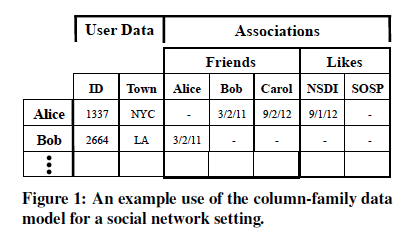
\includegraphics[scale=0.5]{Figure_Lloyd_ColumnHierarchy.png}
\end{frame}


% --------------------------------------------------- Slide --
\begin{frame}
\frametitle{Eiger: Operations}
\begin{itemize}
\pause \item Cassandra has only 3 operations (key determines row)
	\begin{itemize}
		\item Insert(table, key, rowMutation)
		\item Get(table, key, columnName)
		\item Delete(table, key, columnName)
	\end{itemize}
\pause \item Eiger adds more complex transactions
	\begin{itemize}
		\item Batch Mutate
		\item Atomic Mutate
		\item Multiget Slice
	\end{itemize}	
\end{itemize}  
\end{frame}

% --------------------------------------------------- Slide --
\begin{frame}
\frametitle{Eiger: Read Algorithm}
\begin{itemize}
\pause \item Non-blocking
\pause \item Partition Tolerant
\end{itemize}  
\end{frame}

% --------------------------------------------------- Slide --
\begin{frame}
\frametitle{Eiger: Read Algorithm}
\begin{itemize}
\pause \item Example
\end{itemize}  
\end{frame}

% --------------------------------------------------- Slide --
\begin{frame}
\frametitle{Eiger: Write Algorithm}
\begin{itemize}
\pause \item Atomically write set of keys
\pause \item Lock free (and thus low latency)
\pause \item Does not block concurrent reads
\end{itemize}  
\end{frame}

% --------------------------------------------------- Slide --
\begin{frame}
\frametitle{Eiger: Write Algorithm}
\begin{itemize}
	\item Example:
\end{itemize}  
\end{frame}




% --------------------------------------------------- Slide --
\begin{frame}
\frametitle{Evaluation}
\begin{itemize}
\pause \item Comparison to Cassandra
		\begin{itemize}
			\item Within 7\% of throughput Using Facebook-like data
			\begin{itemize}
				\item Ops/sec
				\item Keys/sec
				\item Columns/sec
			\end{itemize}
		\end{itemize}
\end{itemize}  
\end{frame}

% --------------------------------------------------- Slide --
\begin{frame}
\frametitle{Related Research}
\begin{itemize}
\pause \item Mahajan et al. showed that Causal Consistency strongest that guarantees low latency.
\end{itemize}  
\end{frame}

% --------------------------------------------------- Slide --
\begin{frame}
\frametitle{Conclusion: Relationship between 2 Papers}
\begin{itemize}
\pause \item Similarities
	\begin{itemize}
		\item Geo-replicated Systems
		\item Provide consistency
		\item Decrease latencies
	\end{itemize}
\pause \item Differences
	\begin{itemize}
		\item Li: Latency versus Consistency.
			\begin{itemize}
				\item Separate operations into those that must be consistent and those that need not.
			\end{itemize}
		\item Lloyd: Consistency versus Throughput (requiring low latency)
			\begin{itemize}
				\item Extend previous system to offer causal consistency with small hit to throughput.
			\end{itemize}
	\end{itemize}

\end{itemize}  
\end{frame}


% --------------------------------------------------- Slide --

\section{Bibliography} 

\begin{frame}
\frametitle{Bibliography}


%%% SHANNON'S REFERENCES
\begin{itemize}
\item \textbf{Stronger Semantics for Low-Latency Geo-Replicated Storage}, 
\textit{Proceedings of the 10th USENIX Symposium on Networked Systems Design and Implementation (NSDI’13)}, 
Wyatt Lloyd, Michael J. Freedman, Michael Kaminsky, and David G. Andersen, 
April 2013

\item \textbf{Out in the Open: The Abandoned Facebook Tech That Now Helps Power Apple}, 
\textit{www.wired.com}
, Klint Finley, Aug. 4, 2014

\item \textbf{A Short Primer on Causal Consistency}, 
\textit{;login: The Usenix Magazine Volume 38, Number 4}, 
Wyatt Lloyd, Michael J. Freedman, Michael Kaminsky, and David G. Andersen, , August 2013

\item \textbf{Netflix's Viewing Data: How We Know Where You Are in House of Cards},
\textit{http://techblog.netflix.com/search/label/Cassandra}
January 27, 2015



\end{itemize}  
\end{frame}


\begin{frame}
\frametitle{Bibliography}

\begin{itemize}
\item \textit{http://wiki.apache.org/cassandra}

\end{itemize}  
\end{frame}




\end{document} 